\documentclass[a4paper]{article}
\usepackage[utf8x]{inputenc}
\usepackage[T1,T2A]{fontenc}
\usepackage[russian]{babel}
\usepackage{hyperref}
\usepackage{indentfirst}
\usepackage{listings}
\usepackage{color}
\usepackage{here}
\usepackage{array}
\usepackage{multirow}
\usepackage{graphicx}

\usepackage{caption}
\renewcommand{\lstlistingname}{Программа} % заголовок листингов кода

\usepackage{listings}
\lstset{ %
extendedchars=\true,
keepspaces=true,
language=bash,					% choose the language of the code
basicstyle=\footnotesize,		% the size of the fonts that are used for the code
numbers=left,					% where to put the line-numbers
numberstyle=\footnotesize,		% the size of the fonts that are used for the line-numbers
stepnumber=1,					% the step between two line-numbers. If it is 1 each line will be numbered
numbersep=5pt,					% how far the line-numbers are from the code
backgroundcolor=\color{white},	% choose the background color. You must add \usepackage{color}
showspaces=false				% show spaces adding particular underscores
showstringspaces=false,			% underline spaces within strings
showtabs=false,					% show tabs within strings adding particular underscores
frame=single,           		% adds a frame around the code
tabsize=2,						% sets default tabsize to 2 spaces
captionpos=b,					% sets the caption-position to bottom
breaklines=true,				% sets automatic line breaking
breakatwhitespace=false,		% sets if automatic breaks should only happen at whitespace
escapeinside={\%*}{*)},			% if you want to add a comment within your code
postbreak=\raisebox{0ex}[0ex][0ex]{\ensuremath{\color{red}\hookrightarrow\space}}
}

\usepackage[left=2cm,right=2cm,
top=2cm,bottom=2cm,bindingoffset=0cm]{geometry}

\begin{document}	% начало документа

\begin{titlepage}	% начало титульной страницы

	\begin{center}		% выравнивание по центру

		\large Санкт-Петербургский Политехнический Университет Петра Великого\\
		\large Институт компьютерных наук и технологий \\
		\large Кафедра компьютерных систем и программных технологий\\[6cm]
		% название института, затем отступ 6см
		
		\huge Программирование\\[0.5cm] % название работы, затем отступ 0,5см
		\large Отчет по курсовой работе \\[0.1cm]
		\large Приложение "Курсы валют"\\[5cm]

	\end{center}


	\begin{flushright} % выравнивание по правому краю
		\begin{minipage}{0.25\textwidth} % врезка в половину ширины текста
			\begin{flushleft} % выровнять её содержимое по левому краю

				\large\textbf{Работу выполнила:}\\
				\large Власова А.В.\\
				\large {Группа:} 23501/4\\
				
				\large \textbf{Преподаватель:}\\
				\large Вылегжанина К.Д.

			\end{flushleft}
		\end{minipage}
	\end{flushright}
	
	\vfill % заполнить всё доступное ниже пространство

	\begin{center}
	\large Санкт-Петербург\\
	\large \the\year % вывести дату
	\end{center} % закончить выравнивание по центру

\thispagestyle{empty} % не нумеровать страницу
\end{titlepage} % конец титульной страницы

\vfill % заполнить всё доступное ниже пространство








% Содержание
\tableofcontents
\newpage



\section{Проектирование приложения для отслеживания курсов валют}

В современном мире деньги играют важную роль в жизни каждого человека. Людям, которые планируют выезжать за границу или собираются покупать валюту и размещать ее на вклад, необходимо знать текущий курс той или иной валюты. Отслеживать валютные курсы можно на финансовых телеканалах, на информационных порталах, а также с помощью специальных приложений. В связи с тем, что сейчас информация о курсах валют является востребованной, было решено создать приложение, которое позволило бы пользователям получать данные об основных мировых валютах.   

\subsection{Задание}

Разработать приложение, позволяющее пользователям получать текущие курсы валют, отслеживать их изменения за определенный промежуток времени, а также конвертировать мировые валюты.

\subsection{Концепция}

Готовое приложение дает возможность пользователям получать информацию о текущих курсах валют, отслеживать динамику их изменения за указанный период и конвертировать денежные валюты. Для удобства работы пользователя программа оснащена графическим интерфейсом.

\subsection{Минимально работоспособный продукт}

Графическое приложение, предназначенное для получения текущих курсов валют, отслеживания динамики их изменения и конвертирования мировых валют.

\subsection{Выделенные подпроекты}

В процессе проектирования приложения было выделено три подпроекта.

\begin{itemize}

\item \textbf{Core}

Библиотека, представляющая бизнес-логику приложения.

\item \textbf{Console}

Консольное приложение, предоставляющее возможность взаимодействия пользователя с ядром через консоль.

\item \textbf{GUI}

Приложение, предоставляющее пользователю графический интерфейс для взаимодействия с ядром.

\end{itemize}

\subsection{Описание интерфейса библиотеки}

Интерфейс библиотеки содержит в себе следующие методы:

\begin{itemize}

\item Метод, возвращающий курс заданной валюты на сегодня

\textbf{double getExchange(CurrenciesNames name);}

\item Метод, возвращающий курс заданной валюты на определенную дату

\textbf{double getExchange(CurrenciesNames name, String date);}

\item Метод, возвращающий курсы всех доступных валют на сегодня

\textbf{List<Currency> getAllExchanges();}

\item Метод, возвращающий курсы всех доступных валют на заданную дату

\textbf{List<Currency> getAllExchanges(String date);}

\item Метод, позволяющий конвертировать валюты

\textbf{double convert(CurrenciesNames originalCurrency, CurrenciesNames finalCurrency, double number);}

\item Метод, возвращающий статистику изменения курса валюты за указанный период

\textbf{List<Currency> getStatistics(CurrenciesNames currency, String period);}

\end{itemize}

\subsection{Выводы}

В данном разделе рассмотрен процесс проектирования приложения для отслеживания курсов валют. Описаны концепция приложения и минимально работоспособный продукт, перечислены выделенные подпроекты, а также описаны методы, входящие в интерфейс библиотеки. 

\section{Реализация приложения для отслеживания курсов валют}

\subsection{Среда разработки}

Операционная система: Windows 8

Среда разработки: IntelliJ IDEA 2016.2.4

Компилятор: javac, \verb|JDK 1.8.0_102|

\subsection{Выделенные классы}

В библиотеке были выделены следующие классы:
\begin{itemize}

\item \textbf{CurrenciesNames}  - перечисление доступных валют.

\item \textbf{Currency} - содержит основную информацию о валюте. Позволяет получить курс валюты и дату, когда этот курс был действителен, узнать, как изменился курс по сравнению с предыдущим днем, а также получить буквенный код валюты и ее русское название.

\item \textbf{HTMLParser} - устанавливает соединение с сайтом cbr.ru. Содержит метод, возвращающий курс заданной валюты. 


\item \textbf{Day} - класс для работы с датами. Содержит методы, возвращающие нужную дату в отформатированном виде.

\item \textbf{ExchangeRatesAPI} - интерфейс библиотеки. Описан в предыдущем разделе.

\item \textbf{ExchangeRates} - реализует интерфейс библиотеки. 

\end{itemize}

В подпроекте \textbf{Console} выделен единственный класс \textbf{Application}, обеспечивающий взаимодействие пользователя с ядром через консоль. Содержит в себе методы, позволяющие выводить в консоль курс заданной валюты на сегодня и на заданную дату, курсы всех валют одновременно, а также конвертировать валюты.\\


Проект \textbf{GUI} содержит в себе четыре класса:

\begin{itemize}

\item \textbf{ExchangeRatesGUI} - окно приложения, содержащее панель кнопок для переключения между панелями, реализованными в других классах.

\item \textbf{Rates} - панель, на которой вырисовывается таблица с курсами валют.

\item \textbf{Converter} - панель, содержащая конвертер валют.

\item \textbf{Statistics} - панель, на которой отображается таблица, описывающая динамику изменения определенной валюты за указанный период. 

\end{itemize}

\subsection{Примеры работы консольного приложения}

Для демонстрации работы консольного приложения ниже представлены снимки экрана работающего приложения.

\begin{figure}[H]
	\begin{center}
		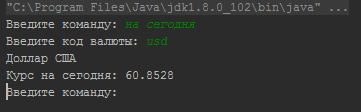
\includegraphics[scale=1.2]{screen/console_1.png}
		\caption{Вывод курса на сегодня} 
		\label{pic: console main menu} % название для ссылок внутри кода
	\end{center}
\end{figure} 

\begin{figure}[H]
	\begin{center}
		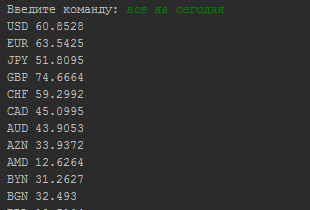
\includegraphics[scale=1.2]{screen/console_2.png}
		\caption{Вывод всех курсов на сегодня} 
		\label{pic:pic_name} % название для ссылок внутри кода
	\end{center}
\end{figure}

\begin{figure}[H]
	\begin{center}
		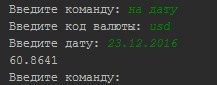
\includegraphics[scale=1.3]{screen/console_3.png}
		\caption{Вывод курса на заданную дату} 
		\label{pic:pic_name} % название для ссылок внутри кода
	\end{center}
\end{figure}

\begin{figure}[H]
	\begin{center}
		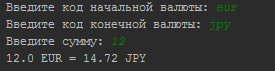
\includegraphics[scale=1.2]{screen/console_4.png}
		\caption{Конвертирование валюты} 
		\label{pic:pic_name} % название для ссылок внутри кода
	\end{center}
\end{figure}

\newpage

\subsection{Пример работы графического приложения}

Ниже приведены снимки экрана для демонстрации работы графического приложения.

\begin{figure}[H]
	\begin{center}
		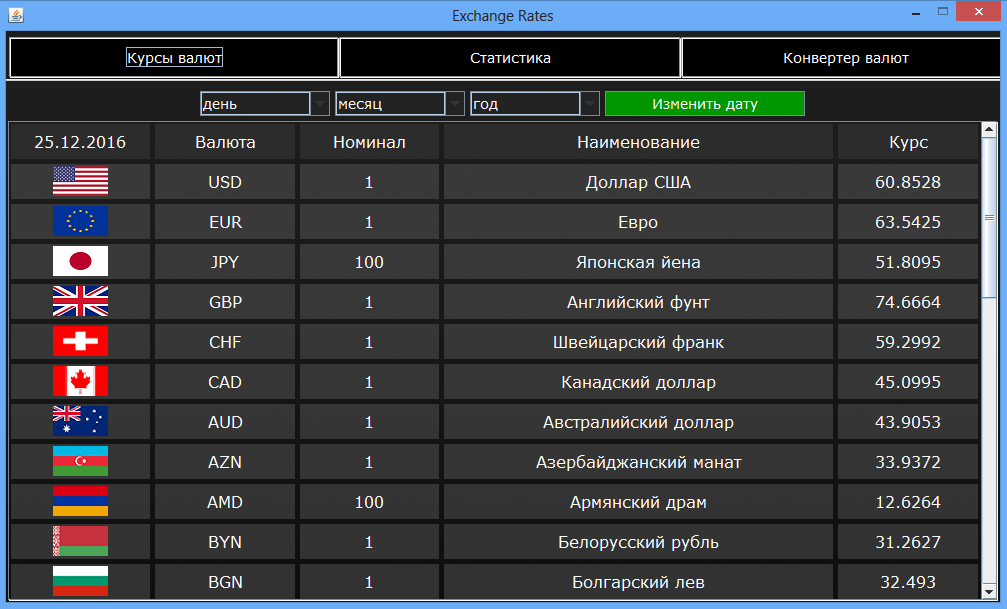
\includegraphics[scale = 0.7]{screen/GUI_1.png}
		\caption{Таблица с курсами} 
		\label{pic:pic_name} % название для ссылок внутри кода
	\end{center}
\end{figure}

\begin{figure}[H]
	\begin{center}
		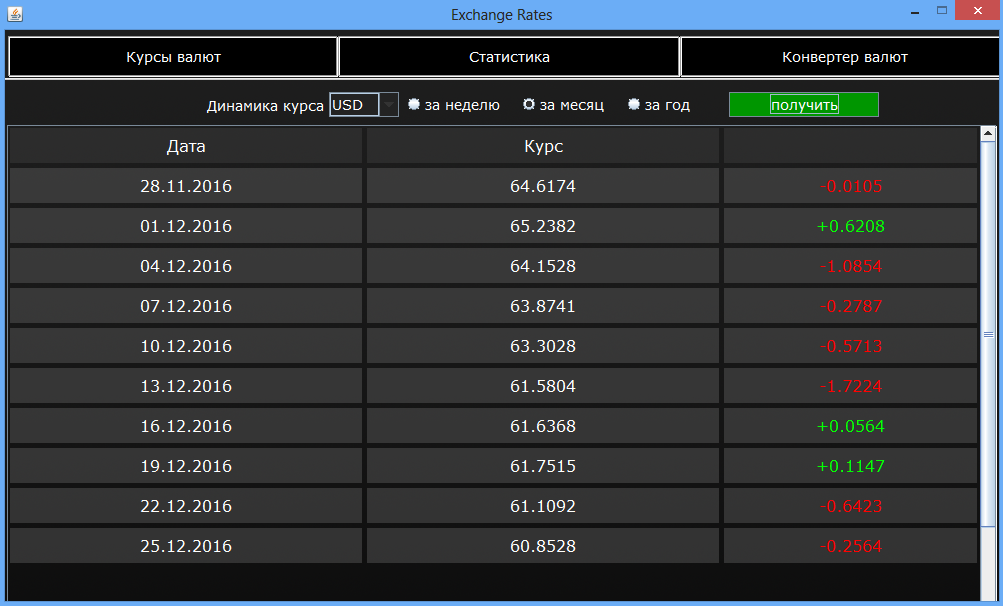
\includegraphics[scale = 0.7]{screen/GUI_2.png}
		\caption{Изменение курса USD} 
		\label{pic:pic_name} % название для ссылок внутри кода
	\end{center}
\end{figure}

\begin{figure}[H]
	\begin{center}
		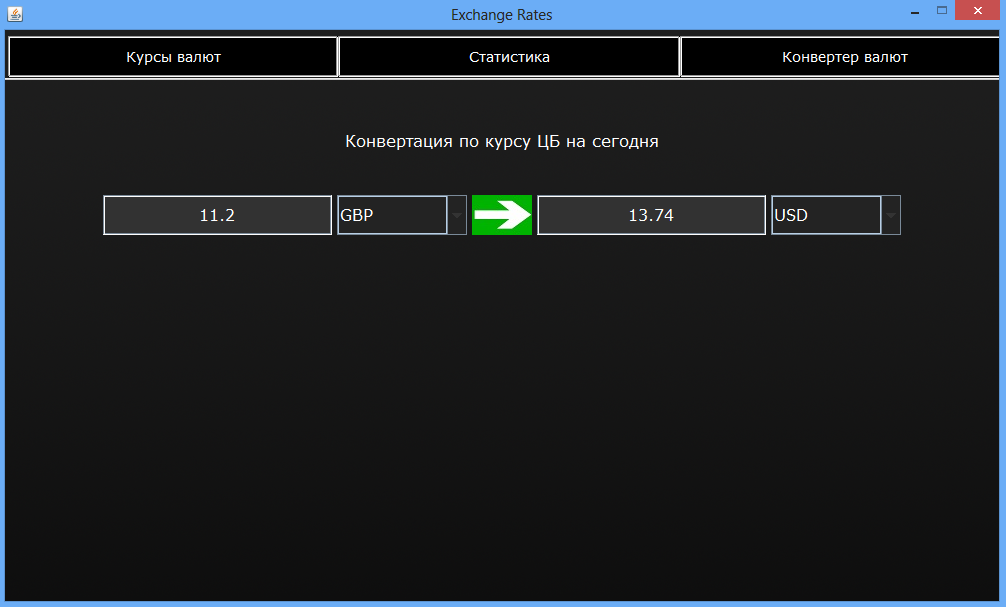
\includegraphics[scale = 0.7]{screen/GUI_3.png}
		\caption{Конвертирование валют} 
		\label{pic:pic_name} % название для ссылок внутри кода
	\end{center}
\end{figure}

\subsection{Выводы}

В данном разделе были описаны все классы, выделенные в процессе работы над проектом. Также были сделаны снимки экрана, демонстрирующие работу консольного и графического приложений.

\section{Процесс обеспечения качества и тестирование}

\subsection{Просмотр кода и демонстрации}

Для обнаружения ошибок в коде программы один раз был проведен просмотр кода, замечания по которому практически полностью исправлены. Также была осуществлена демонстрация работы графического приложения.

\subsection{Тестирование}

Для проверки работы библиотеки использовались автоматические тесты, покрывающие основную функциональность ядра. Также в процессе разработки приложения проводилось ручное тестирование программы.

\subsection{Выводы}

В данном разделе описаны просмотр кода и демонстрация, проведенные во время разработки приложения, а также процесс тестирования программы. 

\section{Выводы}

В результате работы над курсовым проектом было реализовано приложение, предназначенное для получения информации о курсах валют. В процессе создания приложения получены навыки написания программ на языке Java, изучены основные особенности данного языка, а также приобретен опыт работы с библиотекой для создания графических приложений Swing.   

\section{Приложение 1}

\captionof{lstlisting}{ExchangeRatesAPI.java}
\lstinputlisting{../Core/src/main/java/ru/vlasova/exchangeRates/core/ExchangeRatesAPI.java}
\parindent=1cm

\captionof{lstlisting}{ExchangeRates.java}
\lstinputlisting{../Core/src/main/java/ru/vlasova/exchangeRates/core/ExchangeRates.java}
\parindent=1cm

\captionof{lstlisting}{CurrenciesNames.java}
\lstinputlisting{../Core/src/main/java/ru/vlasova/exchangeRates/core/CurrenciesNames.java}
\parindent=1cm

\captionof{lstlisting}{Currency.java}
\lstinputlisting{../Core/src/main/java/ru/vlasova/exchangeRates/core/Currency.java}
\parindent=1cm

\captionof{lstlisting}{Day.java}
\lstinputlisting{../Core/src/main/java/ru/vlasova/exchangeRates/core/Day.java}
\parindent=1cm

\captionof{lstlisting}{HTMLParser.java}
\lstinputlisting{../Core/src/main/java/ru/vlasova/exchangeRates/core/HTMLParser.java}
\parindent=1cm

\captionof{lstlisting}{IllegalDateFormatException.java}
\lstinputlisting{../Core/src/main/java/ru/vlasova/exchangeRates/core/Exceptions/IllegalDateFormatException.java}
\parindent=1cm

\captionof{lstlisting}{NoSuchCurrencyException.java}
\lstinputlisting{../Core/src/main/java/ru/vlasova/exchangeRates/core/Exceptions/NoSuchCurrencyException.java}
\parindent=1cm

\captionof{lstlisting}{CurrencyTest.java}
\lstinputlisting{../Core/src/test/java/ru/vlasova/exchangeRates/core/CurrencyTest.java}
\parindent=1cm

\captionof{lstlisting}{DayTest.java}
\lstinputlisting{../Core/src/test/java/ru/vlasova/exchangeRates/core/DayTest.java}
\parindent=1cm

\captionof{lstlisting}{ExchangeRatesTest.java}
\lstinputlisting{../Core/src/test/java/ru/vlasova/exchangeRates/core/ExchangeRatesTest.java}
\parindent=1cm

\captionof{lstlisting}{HTMLParserTest.java}
\lstinputlisting{../Core/src/test/java/ru/vlasova/exchangeRates/core/HTMLParserTest.java}
\parindent=1cm

\captionof{lstlisting}{Application.java}
\lstinputlisting{../Console/src/java/ru/vlasova/exchangeRates/console/Application.java}
\parindent=1cm

\end{document}